\ignore{
\begin{verbatim}
 * Overview
    High-level exec. semantics
    Coverage wrt threat model
 * Detailed (micro)architecture
    * Buffers
    * ISA extensions
 * Putting it all together
    [Flowcharts?]
    * Behavior under speculation
    * Behavior under non-speculative exec.
    * Relation to value prediction
* Overheads?
* Correctness guarantee?
* New vulnerabilities?
 \end{verbatim}
 }
 
 \begin{figure*}
     \centering
     \subfloat[Slice example]{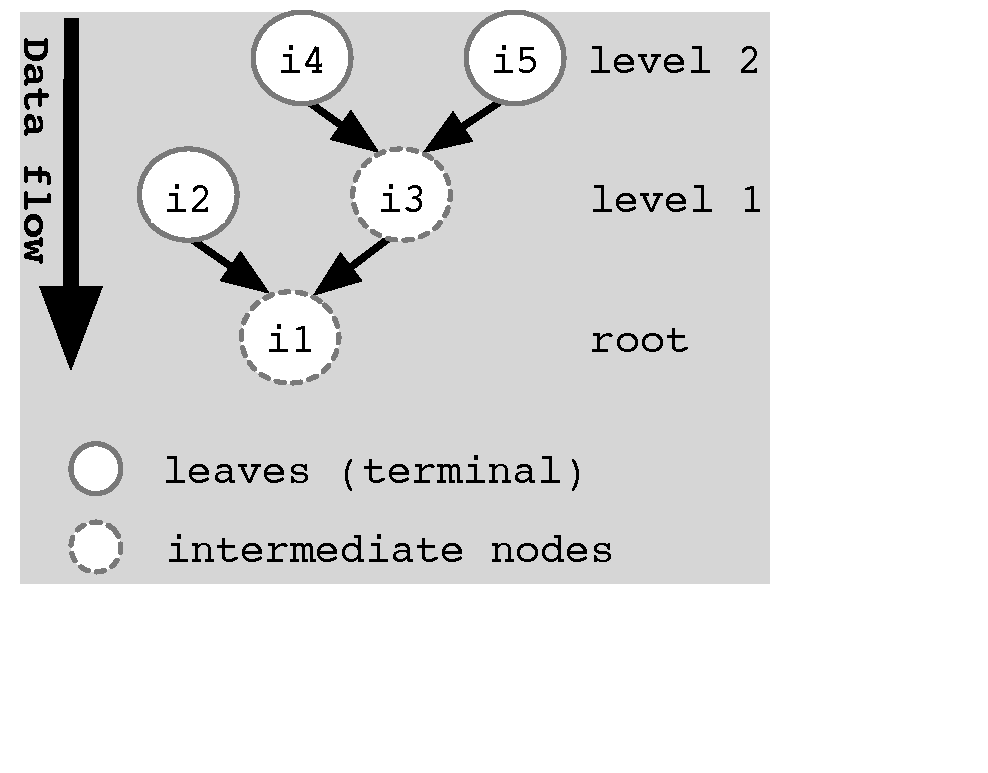
\includegraphics[width=0.25\textwidth]{figs/rt.pdf}\label{fig:rt}}
     ~~~
     \subfloat[Execution semantics and  $\mu$-architecture]{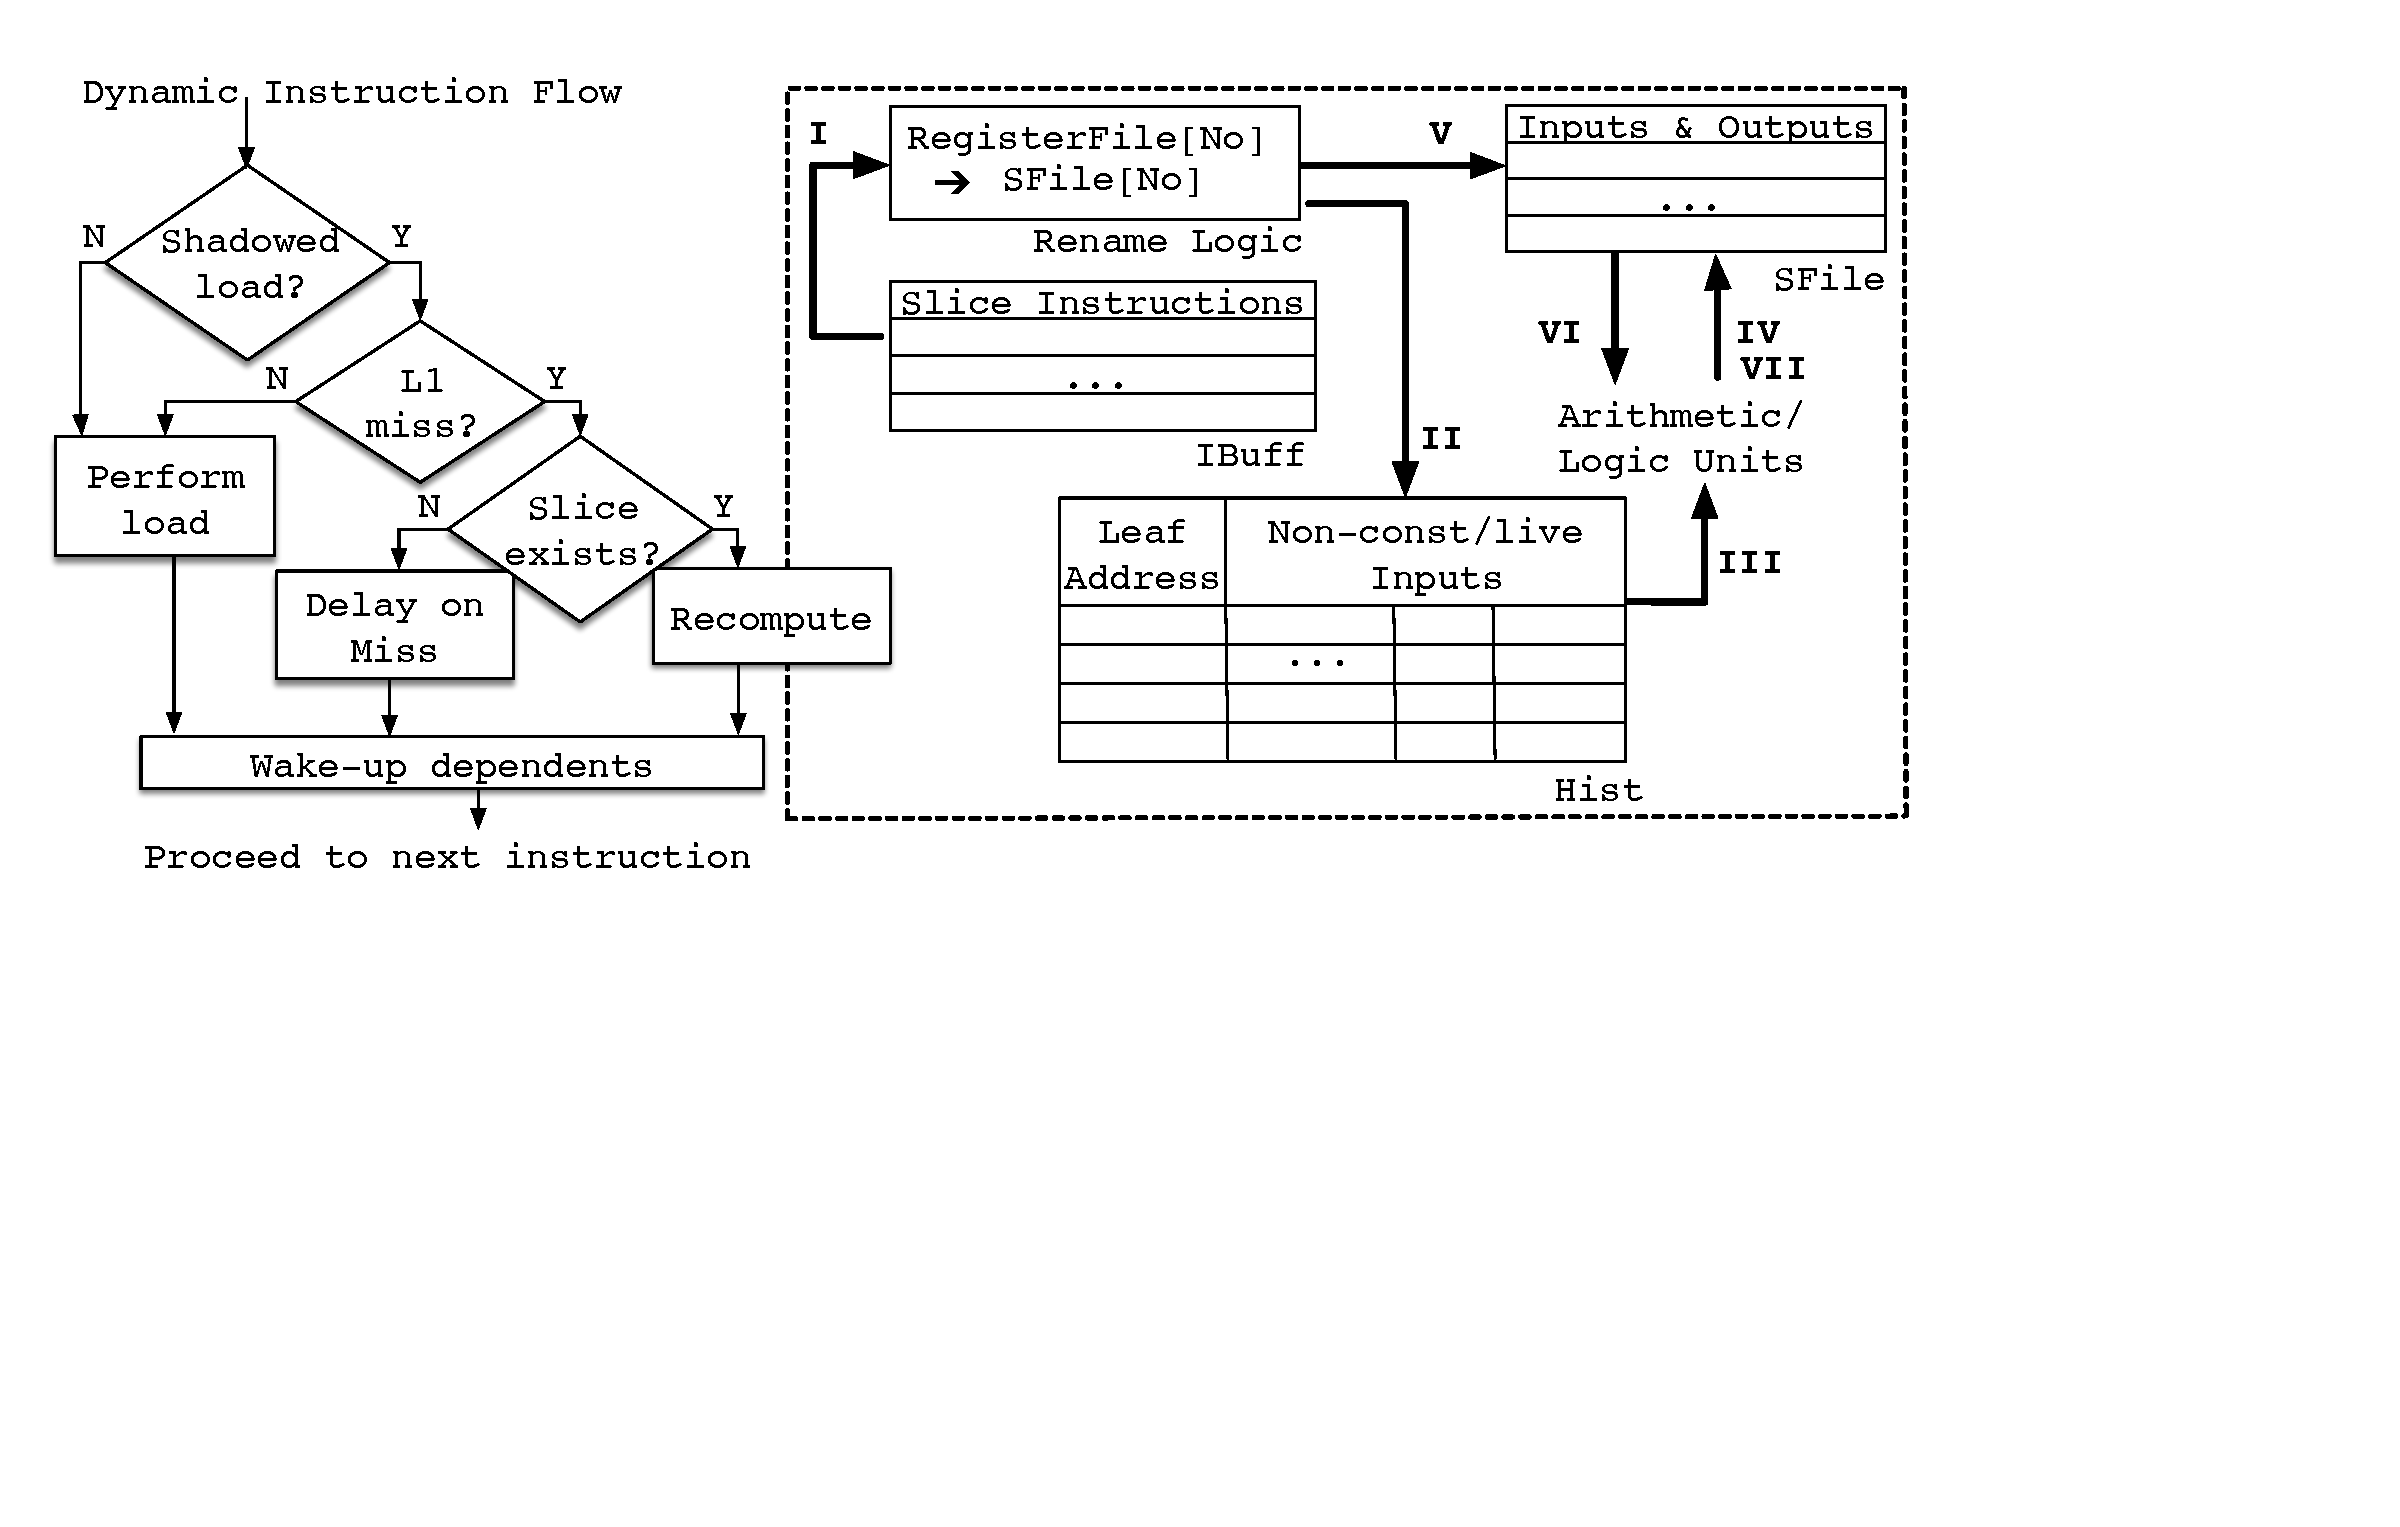
\includegraphics[width=0.65\textwidth]{figs/ctrl.pdf}\label{fig:ctrl}}
     \caption{ \arch\ Overview. All $\mu$-architectural buffers from (b) have  
an $\texttt{invalid}$ field per entry to
manage space (de)allocation.}
     \label{fig:overview}
\vshrink{.2}
\end{figure*}
 
% Overview
 
 \subsection{Execution Semantics}
 
 \arch\ only resorts to recomputation to regenerate values which otherwise would be read from a speculative load from the memory hierarchy, and only so, if the respective speculative load misses in the L1 cache. Recomputation takes place as long as a slice exists and the input operands to the slice instructions can be made readily available at the anticipated time of recomputation. This execution model has the potential of delivering higher energy efficiency, as imbalanced technology scaling renders loads much more energy hungry and slower than arithmetic/logic instructions (which form slices)~\cite{Horow}. 
 %Typically a slice contains \redHL{no more than 10-15 instructions}.
 
%\ignore{
Not all of the input operands of leaf instructions of a slice can be
(re)generated by recomputation.  This may be the case if input operands
correspond to (i) read-only values to be loaded from memory, such as program
inputs; or (ii) register values which are lost, i.e., overwritten at the time of
recomputation. We will refer to such input operands as {\em non-recomputable}
inputs. For \recomp\ to work, non-recomputable inputs of slice leaves
should not only be available at the anticipated time of recomputation, but also
be retrievable in an energy-efficient manner.
%
Recomputation cannot eliminate any memory access to retrieve the
non-recomputable inputs of slice leaves.  If non-recomputable inputs do not
reside in close physical proximity to the processor, the energy cost of their
retrieval may easily exceed the energy cost of memory accesses, rendering recomputation useless.    
Buffering can help in this case. No dedicated buffering is necessary if the leaf input operands
correspond to constants or live register values. 
%}

While \arch\ shares basic microrachitectural structures with Amnesiac~\cite{amnesiac17} to facilitate \recomp\ (such as dedicated buffers to prevent corruption of $\mu$-architectural state during recomputation), its
execution semantics are quite different when it comes to slice formation, triggering recomputation, and committing recomputed values to architectural state. These stem from the subtle difference in optimization targets: Amnesiac uses \recomp\ to maximize energy efficiency irrespective of security implications. \arch, on the other hand, uses \recomp\ to eliminate (already known or yet to be discovered) threats induced by speculative loads. Specifically: 
%Putting it all together, execution semantics are different than Amnesiac~\cite{amnesiac17} in the following ways:
 \begin{itemize}
     \item{\em What to recompute (slice formation):} \arch\ does not impose any direct constraint on slice length to preserve energy efficiency, as opposed to Amnesiac, as we are not after minimizing energy or latency per load. As long as a slice exists, and its inputs can be made readily available at the anticipated time of recomputation, \arch\ would consider it for recomputation. The only practical limitation on slice length may stem from storage overhead of $\mu$-architectural buffers in this case. 
     \item {\em When to recompute:} \arch\ swaps speculative loads that miss in L1 for recomputation (i.e., with producer instructions of the respective value along a slice). Amnesiac on the other hand, triggers recomputation (irrespective of whether the load is speculative or not) only if it is more energy-efficient to do so. 
 %    \item{\em How to recompute?} Similar to Amnesiac, we use dedicated buffers to prevent corruption of $\mu$-architectural state. 
     \item{\em When/how to commit a recomputed value to architectural state:} In Amnesiac, a recomputed value is written into the destination register of the  load before execution resumes from where the corresponding load (which is swapped for recomputing instructions) has left. \arch\ has to keep these values buffered until the speculation is resolved (i.e., all shadows are lifted).  \recomp\ cannot change architectural state under speculation, by definition. {However, just as speculative loads that \emph{hit} in the L1, recomputed loads pass their value (in a physical register) to dependent instructions and advance execution.}  
 \end{itemize}
 
% We will detail design specifics next. 
 
\subsection{Slice Formation \& Annotation}
%\noindent{\bf Slice Formation:}
Similar to Amnesiac, we rely on a compiler pass (backed up by profiling) to form and annotate slices, which 
 mainly constitutes
%first estimates,
%probabilistically 
%(as detailed in the following and Section~\ref{sec:setup}),
%\footnote{Section~\ref{sec:setup} details a representative
%probabilistic model based on memory access statistics collected from profiling.}
%the energy
%consumption of loading $v$, $E_{ld,v}$. Next comes 
%with 
dependency analysis to
identify the producer instructions for each load.
%, in order to calculate the anticipated
%cost of potential recomputation. 
{\color{magenta}  Instead of a compiler, the same job can be performed by \emph{dynamic binary instrumentation} at run time (albeit with probably inferior alias analysis but more dynamic information), rendering recompilation unnecessary in deployments where it is not an option.
Slice creation is \emph{best effort}. Not being able to generate a recomputation slice for a load is not a security weakness, but a performance liability under a security technique such as Delay-on-Miss. As we will see later, no strict guarantees are necessary for the validity of the recomputation as this can be protected at runtime with architectural support.}


This pass builds the slice level by level, where
%This step starts building the slice (where 
the immediate producer of the value to be loaded resides at the root.
%), and lets the slice grow
%level by level. 
As opposed to Amnesiac, in this case the only restriction to slice length can come from slice input or storage requirements. 
%, as long as the cumulative cost of recomputation along \rsv\
%being constructed remains below $E_{ld,v}$.     
If, during the traversal of dependency chains, we encounter other load instructions, we 
%As the compiler traverses the dependency chains, it may hit
%load instructions. In the proof-of-concept implementation, the
%compiler replaces each such load 
replace them recursively with the respective producer instructions. 
%recursively.
This recursive growth can continue until a store to the same address is encountered.
Loads and stores cannot be present 
%as intermediate nodes 
in any slice by definition.
%In fact, stores can never find place in \rsv, and loads can only, if at all,
%appear at the leaves to read non-recomputable input operands.

Once done, we place 
%corresponding 
each such constructed slice into the binary. 
Similar to Amnesiac, to communicate recomputation opportunities to the runtime, we use 
%\noindent {\bf Slice Annotation:}
%\label{sec:isa}
%As a hint for the runtime scheduler, the compiler replaces each load that has a slice
%the swap
%of which with recomputation is likely to be more energy-efficient (according to
%the probabilistic energy cost comparison explained above) 
%with a 
the special control
flow instruction $\texttt{RCMP}$ which semantically corresponds to an atomic bundle of a conditional branch + load (where no prediction is involved for the ``branch'' portion).
%In this manner, the recomputing instance of an
%instruction is separated from its original, ``computing'' instance.
%Semantically, $\texttt{RCMP}$ corresponds to the fusion of a conditional branch
%with a load\footnote{
%Depending on the specifics of the underlying instruction set architecture (ISA),
%$\texttt{RCMP}$ can also be synthesized by a pair of branch and load
%instructions, without loss of generality. 
%}. 
The runtime scheduler resolves the branching condition: If the respective load (while shadowed) misses in L1, $\texttt{RCMP}$ acts as a jump to the entry point (starting from the
leaves) of the corresponding slice. Otherwise (i.e., if the load hits in L1 when shadowed or if the load is not shadowed), $\texttt{RCMP}$ is not any different than a classic load.
All operands of
the respective load and the starting address of its slice form the operands of $\texttt{RCMP}$. 
$\texttt{RTN}$ instruction (similar to procedure return in nature) demarcates the end of each slice and returns the control to the instruction following $\texttt{RCMP}$. Before the return takes place, the recomputed value is provided to the consumers of the respective load, in the same way as if the load was actually performed. However, the destination register of the corresponding load only gets updated after the load becomes non-speculative.
During runtime we can re-order the leaf instructions in a slice in different ways, as leaf instructions cannot
depend on each other. 

%\ignore{
As explained in~\cite{amnesiac17}, recomputation is possible even if the compiler cannot prove that all input operands of
slice leaves correspond to constants or live register values at the anticipated
time of recomputation, by keeping such input operands (e.g., overwritten register values) in a dedicated buffer.
%}

%\ignore{
{\em Only if the leaves of} the slice {\em have non-recomputable input operands},
the compiler places 
%$\texttt{SLC}$ and 
$\texttt{REC}$ instructions into the
binary, which serve buffering of non-recomputable input operands such as
overwritten register values.
%as detailed in Sections~\ref{sec:micro} and~\ref{sec:sched}.  
%An $\texttt{SLC}$ instruction
%goes right before the entry point of \rsv.  $\texttt{SLC}$ has a single integer
%operand, $\texttt{RSlice-ID}$ to carry the unique ID of \rsv.  
An $\texttt{REC}$
instruction goes right after each instruction, a replica of which serves as a
leaf in the slice.  $\texttt{REC}$ has 
%two 
a single integer operand:
%$\texttt{RSlice-ID}$, and 
$\texttt{leaf-address}$ which points to the address of
the respective leaf instruction in the slice.  $\texttt{REC}$ practically checkpoints the input
operands 
%of its predecessor (which form the non-recomputable inputs
%of the leaf at $\texttt{leaf-address}$) 
to a dedicated buffer. 
%}
{\color{magenta} The target address of the producer instruction (e.g., store) is also saved as a tag for the whole slice in this dedicated buffer. This tag can be matched by future stores on the same address, to invalidate the slice (and cancel recomputation).}

\subsection{($\mu$-)Architecture}
%\noindent{\bf $\mu$-Architecture:}
We next detail $\mu$-architectural structures for \arch, as depicted in Fig.~\ref{fig:ctrl}, which serve two main purposes:
(1) Keeping $\mu$-architectural state intact during recomputation; (2) Making 
slice instructions and operands available at the anticipated time of recomputation. 
%All $\mu$-architectural buffers have  
%SFile, Hist, and IBuff all feature 
%an $\texttt{invalid}$ field per entry to
%manage space (de)allocation.

%\ignore{
Fig.~\ref{fig:ctrl} depicts microarchitectural support to meet  {
Condition-I} and {Condition-II} in orchestrating recomputation.  Recall
that, for simplicity, only one slice can be active, i.e., traversed for recomputation, at a
time but that can be rectified with a more elaborate $\mu$-architecture. 
%{\color{red} STEFANOS: I don't understand this restriction. We're just injecting more instructions in the instruction queue. If we encounter another load that can be recomputed we insert more instructions in the IQ and let everything run at max ILP. In other words I do not see the reason why we do not allow RLP (Recompute-Level-Parallelism). Maybe because the call-return semantics of recomputation? Bur even so, we can execute functions in parallel by predicting  their returns!}
%\footnote{Offloading recomputation to spare or idle cores, or using helper threads may improve energy efficiency further by enabling concurrent recomputation. However, the basic proof-of-concept implementation assumes strictly sequential execution semantics.}
%ULYA: Ack. This is coming from our previous analysis which we didn't consider OoO execution in detail. But at the same time, I'd sparee detailed discussion of this for now (unless we want to get deep into microarchitecture here). 
%}

\noindent {\em Scratch-File (SFile)}  practically acts as the physical registerfile during recomputation. 
Specifically, while recomputation is in progress, all data flows through the SFile. Thereby, \arch\ preserves $\mu$-architectural state during recomputation. No structure beyond SFile is necessary in this case, as no memory access instruction is permitted in a slice.

\noindent {\em Rename logic} translates (architectural) register references of slice instructions to SFile entries.
Semantically, it is equivalent to the rename logic of classic out-of-order processors, with SFile replacing the physical registerfile. 

\noindent{\em  Instruction Buffer (IBuff)}
%The dedicated instruction buffer IBuff 
caches slice instructions in order to avoid
%within each slice, in order to relax {\color{red} ISER} amnesic execution's 
unnecessary pressure on the instruction cache.
Each entry of IBuff corresponds to a recomputing instruction. Fetch logic fills IBuff, similar to instruction cache. IBuff feeds the rename logic. 
%once the traversal of (i.e, recomputation along) an \rs\ finishes.  

%\ignore{
\noindent {\em History Table (Hist):} 
For each slice  where the leaf input operands correspond to constants or live
values from the (physical) registerfile, {Condition-II} is automatically
satisfied.  Only for non-recomputable leaf input operands, dedicated storage is
required to satisfy {Condition-II}. The amnesic microarchitecture can buffer
non-recomputable input operands for each slice leaf in the dedicated history
table Hist.
%, upon the first encounter 
%during dynamic execution.  
Each entry of Hist 
%corresponds to an \rs\ leaf, and 
keeps the address ($\texttt{leaf-address}$) and non-recomputable input operands of a leaf
instruction.
%\begin{list}{\labelitemi}{\leftmargin=1em}
%\vshrink{0.2}
%  \itemsep-0.3em 
%  \item the \texttt{RSlice-ID} of the \rs\ the leaf belongs to;
%  \item 
%the address of the leaf instruction;
%  \item the input operand values of the leaf instruction. 
%\vshrink{0.15} 
%\end{list}
%}
{\color{magenta} Hist entries are invalidated if a slice target address tag is matched by a future store (see \autoref{sec:coherence} and \autoref{sec:consistency}) as recomputation in this case can possibly produce an invalid (incoherent) result.
Since this is a rare occurrence, we optimize for the case when this is does not happen: A Bloom filter encodes all the slice tags (target addresses) and if a future store hits in the Bloom filter, the entire Hist and Bloom filter are reset and need to be repopulated anew. See \autoref{sec:coherence} and \autoref{sec:consistency} for more details.}

As opposed to Amnesiac, for \arch, $\texttt{RCMP}$ always translates into $\texttt{branch on L1 miss}$ for speculative loads. 
As shown in Fig.\ref{fig:ctrl}, for each $\texttt{RCMP}$ instruction encountered, \arch\ first checks whether the corresponding load is speculative, and if so, whether it misses in L1. \arch\ triggers recomputation for any shadowed load that misses in L1.
%, by setting a flag. 
Before recomputation starts, \arch\ allocates a physical register where the value to be recomputed goes after recomputation is done\footnote{This register corresponds to the renamed destination register of the respective load, were the load performed instead of recomputation.}.  
Then, control jumps to the entry point of the corresponding slice, and instruction fetch starts from the leaves, one at a time (step $\textbf{II}$). For leaf instructions, the next step ($\textbf{III}$) is renaming the destination register. 
Leaf instructions with constant or live
register input operands do not need to probe any dedicated buffer\footnote{As explained in~\cite{amnesiac17}, recomputation is possible even if the compiler cannot prove that all input operands of
slice leaves correspond to constants or live register values at the anticipated
time of recomputation, by keeping such input operands (e.g., overwritten register values) in a dedicated buffer. If this is the case, leaf instructions will collect their input operands from this buffer.
}.  
%
Non-leaf instructions, on the other hand, 
read their input operands directly from SFile ($\textbf{IV}$)
after having both, the
source and destination registers renamed ($\textbf{III}$).
Upon finishing execution, each slice instruction (irrespective of the level) writes
its result back to the SFile ($\textbf{V}$). 
This process continues until hitting $\texttt{RTN}$. Before return, \arch\ wakes-up consumers of the recomputed value, and copies the value itself to the physical destination register (which would be allocated for the corresponding load, was recomputation not the case).  The recomputed value  waits there for commit until all of its shadows are revoked. 

\ignore{
\subsection{Overheads}
 
During traversal of a slice, latency per recomputing instruction remains very
similar to its classic counterpart, as the amnesic microarchitecture follows the
pipelining semantics of the underlying microarchitecture (just with an
alternative instruction and operand supply of similar latency).

The storage complexity of {\color{red} ISER} amnesic structures from Fig.~\ref{fig:ctrl} tends to
be low \redHL{(Section~\ref{sec:eval})}.  Only the unlikely capacity overflow of Hist
can impair recomputation, and only for slices with non-recomputable leaf input
operands. The amnesic scheduler can track these cases by failed $\texttt{REC}$
instructions  and enforce the corresponding
$\texttt{RCMP}$ to skip recomputation (i.e., to perform the load).  To this end,
the {\color{red} ISER} amnesic scheduler has to uniquely identify the matching $\texttt{RCMP}$.
This can be achieved by assigning  a unique ID, $\texttt{RSlice-ID}$, to each
\rs\ in the binary, and providing it as an operand to both $\texttt{REC}$ and
$\texttt{RCMP}$.

In processing recomputing instructions, the {\color{red} ISER} amnesic microarchitecture has to
differentiate between leaves and intermediate nodes, since different structures
supply the input source operands to each: The inputs of leaves can come from the
registerfile (a live value) or Hist (an overwritten value). The inputs of
intermediate nodes come from SFile. The compiler annotates leaves and accesses
to Hist to distinguish between these cases. Specifically, the compiler changes
source register identifiers of leaf instructions reading their operands from
Hist to an invalid number. Leaf instructions with valid source register
identifiers directly access the registerfile. Non-leaf recomputing instructions
follow the paths \raisebox{0.5pt}{\textcircled{{\raisebox{-0.9pt}{2}}}} and
\raisebox{0.5pt}{\textcircled{{\raisebox{-0.9pt}{6}}}} in Fig.~\ref{fig:ctrl}.

Recall that there is another potential class of leaves with non-recomputable input
operands: read-only values to be loaded from memory, such as program
inputs. In principle, replacing the load to read $v$ from memory with the corresponding slice
which features possibly more than one such load at the leaves does not make sense.
Hist is designated to record overwritten register input operands, but Hist 
can also keep such read-only values, and may make recomputation along such
a slice energy-efficient.  

\redHL{Storage overhead?}
}

\subsection{Limitations \& Side Effects}
 
 \noindent {\em Overhead:} 
 Latency or energy per recomputing instruction embedded into a slice is not any different than the non-recomputing, conventional counterparts. The only difference is that \arch\ executes these extra instructions using a dedicated instruction and data supply rather than the conventional instruction cache and physical registerfile/data cache. There is no fundamental limitation to have multiple slices  in flight simultaneously. The only restriction is practical, as aggressive slice-level parallelism (SLP) would demand a larger IBuff and SFile. 
 IBuff grows with the product of {\em highest degree of slice-level parallelism anticipated, max(SLP)} and {\em (maximum) number of instructions per slice}, where max(SLP) captures the maximum number of slices that can be in flight simulteneously to exploit more ILP via slice-level parallelism. SFile's storage complexity differs from this product only by a constant factor, which is the {\em maximum number of renaming requests per slice instruction} (which, e.g., would be 3 considering a RISC-like ISA, for two sources and one destination register).

 \noindent {\em Coverage:}
 We cannot mathematically guarantee that all speculative loads missing in L1 have a corresponding slice. This may be due to complex producer-consumer chains which cannot be expressed by a chain of arithmetic/logic instructions only and/or slice inputs which cannot be guaranteed to be available at the anticipated time of recomputation. 
 
\noindent {\em Locality:}
Any speculative load that misses in L1 and gets replaced with recomputation would never reach the memory hierarchy. As a result, subsequent memory requests to the same address become more likely to miss in the cache hierarchy, as well. This adverse effect can easily degrade performance, but recomputation targeting such new misses may be able to recover some of the lost performance.
 
\noindent {\em Exception Handling (during Recomputation):}
Exception handling during recomputation is similar to exception handling
under speculation: record exceptions during recomputation and defer their handling after recomputation finishes.
Contrary to speculation, however, recomputation modifies the $\mu$-architectural control flow by executing extra
instructions.  
%\redHL{Shall we ignore/expand this?}

 %\subsection{Vulnerabilities} 
 % Need coherence/consistency discussion for this
 
% \redHL{Ignore vs. expand coverage/exceptions/...?}
 
%\section{Stranger Things} % Remove Before Flight: if this is not an autonomous section distribute its contents appropriately 
\label{sec:stranger-things}
\begin{verbatim}
* Stranger Things go here for the moment 
until we figure out what to do with them.
 \end{verbatim}


\subsection{Coherence and Consistency}
On TSO:
RC seems to work wonders. This is because when we recompute,
the result is by definition correct --- we do not verify.
In this respect TSO is not violated by something that cannot change (see
the ISCA'17 "Non-speculative Load-Load reordering in TSO").
The situation is clear if the recomputation starts off from constants to
compute a new value. The new value is immutable by other cores.
That's what TSO wants.

If the recomputation starts off from values loaded from the L1 (e.g.,
hits) then we must make sure that these values do not change.
But that's easy to do: we must ensure lock-downs (ISCA'17) for these
loads. We can discuss how secure is that, but I believe we can claim
that we can do RC that respects TSO even in this case. 

When we use a real RC, the compiler detects the posibility of recomputation if all the inputs are constants (or pseudo-constant (write-once)?). In this case TSO is correct. The compiler is giving us the guarantee.

The problem may come from 2 sources:

- 1. The compiler does not know well (may-alias) if an input is constant.

- 2. Parallel applications make it worse the first case.

The idea could be to "predict at compiler time" no alias, and add ISCA'17 checks and guarantees at runtime.

Right now, I would go for our current solution. In case of alias we do not recompute(we lose coverage), and we do not add speculation there. -- We can speculate in sw and fix it in hw for a follow up paper.

Note: the compiler cannot guarantee DRF for x86 code, as the model is release consistency instead. 



